\documentclass{article}
\usepackage[margin=1in]{geometry}
\usepackage{graphicx}
\usepackage{xcolor}
\usepackage{float}
\usepackage{amsmath}
\usepackage{cite}
\usepackage{hyperref}
\usepackage{indentfirst}
\graphicspath{{..} {./images}}

\definecolor{navy-blue}{rgb}{0.22,0.38,0.71}

\renewcommand{\contentsname}{\vspace*{-2\baselineskip}}

\hypersetup{
	colorlinks,
	linkcolor=black,
	urlcolor=blue,
	citecolor=black
}
  		
\begin{document}
\begin{titlepage}
	\centering
	{\huge Lab 5 - Digital Modulation: Symbol Synchronization}\\[0.25 in]
	
\includegraphics[width=0.6\textwidth]{ua_logo.png}\\[0.25 in]
	{\large \textbf{ECE 531 - Software Defined Radio\\[0.25 in]
	April 4, 2025\\[0.25 in]}}
	{\large Owen Sowatzke, osowatzke@arizona.edu\\[0.05 in]
	Department of Electrical \& Computer Engineering\\[0.05 in]
	University of Arizona, Tucson, AZ 85721\\[0.5 in]}
	\hypersetup{linkcolor=navy-blue}
	\noindent\hrulefill
	\tableofcontents
	\noindent\hrulefill
\end{titlepage}

% \setlength{\parindent}{0pt}

\section{Introduction}
%Introduction to the laboratory experiment, including a brief description of the objectives and goals.

\section{Procedure}
% Detailed explanation of the laboratory experiment, including the design, implementation, and testing of the system.

\section{Results}
% Results and discussion of the laboratory experiment, including captured outputs, observations, and responses to laboratory questions.

\subsection{Pulse Shaping and Matched Filtering}

Type I Nyquist filters are defined by a rectangular pulse in the frequency domain and a sinc pulse in the time domain. The sinc pulse has zero crossings at $nT$, which produces zero ISI. Because Type I Nyquist filters are a rectangular pulse in the frequency-domain, they have the minimum bandwidth and maximize spectral efficiency. However, there are a couple problems with type I Nyquist filters. First, they are infinite in time. Second, accurate sampling is required. Small timing errors can result in large ISI because the impulse response of a sinc filter decays with $1/t$, which does not converge.

Type II Nyquist filters also have zero crossing at $nT$. However, they have a bandwidth larger than the minimum bandwidth, which allows them to achieve lower ISI sensitivity than type I Nyquist filters. The raised cosine filter is an example of a type II Nyquist filter. Its impulse responses decays with $1/t^3$, which quickly converges in the presence of timing errors.

Next, we compare the frequency response of the SRRC filters for $\beta \in [0,0.1,0.25,0.5,1]$. These frequency responses for these filters are captured in Figures \ref{fig::srrc_freq_response_beta_0} - \ref{fig::srrc_freq_response_beta_1}.

\begin{figure}[H]
	\centerline{\fbox{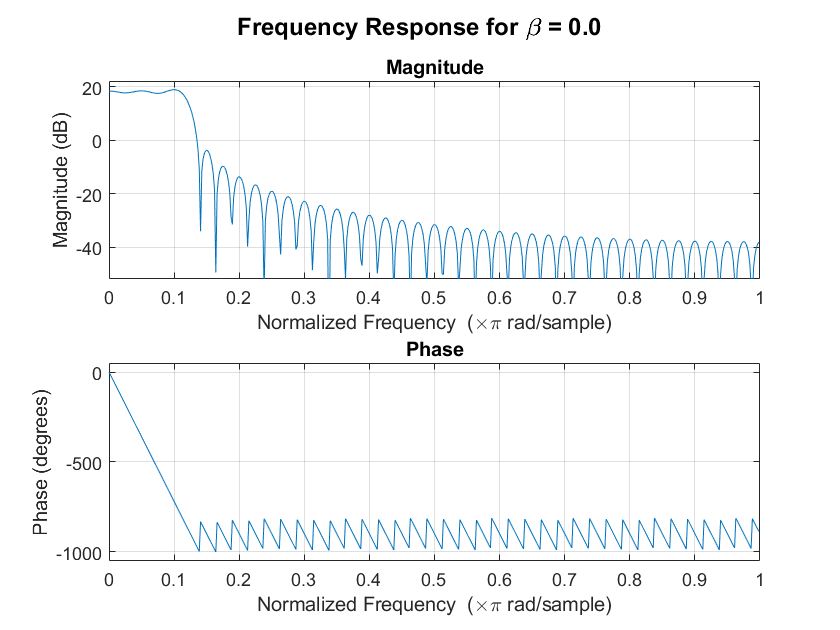
\includegraphics[width=0.5\textwidth]{srrc_freq_response_beta_0.png}}}
	\caption{SRRC Filter Frequency Response with $\beta=0$}
	\label{fig::srrc_freq_response_beta_0}
\end{figure}

\begin{figure}[H]
	\centerline{\fbox{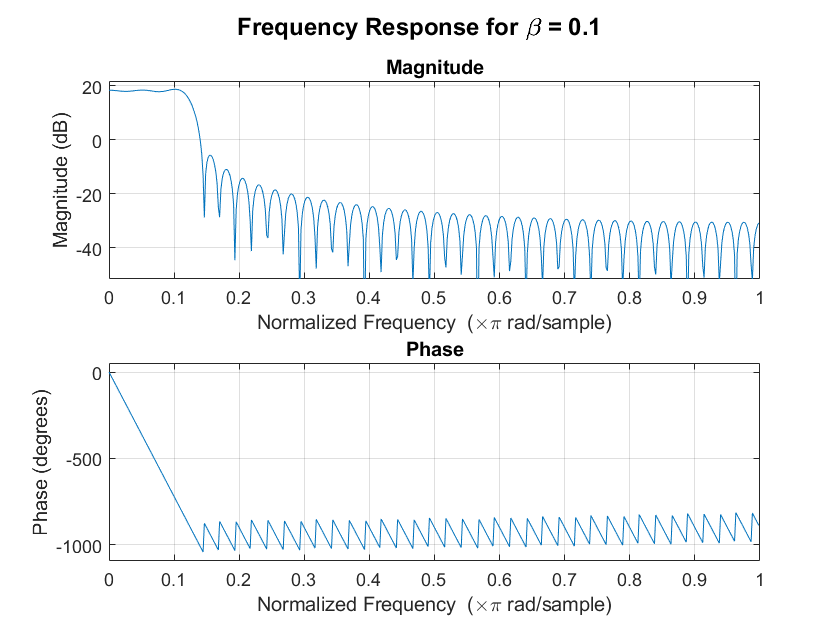
\includegraphics[width=0.5\textwidth]{srrc_freq_response_beta_0_1.png}}}
	\caption{SRRC Filter Frequency Response with $\beta=0.1$}
	\label{fig::srrc_freq_response_beta_0_1}
\end{figure}

\begin{figure}[H]
	\centerline{\fbox{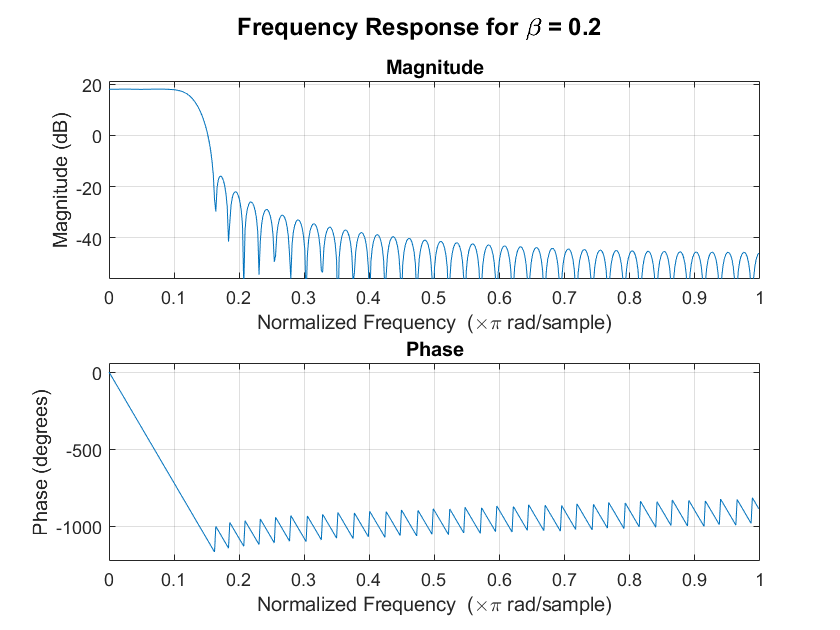
\includegraphics[width=0.5\textwidth]{srrc_freq_response_beta_0_2.png}}}
	\caption{SRRC Filter Frequency Response with $\beta=0.2$}
	\label{fig::srrc_freq_response_beta_0_2}
\end{figure}

\begin{figure}[H]
	\centerline{\fbox{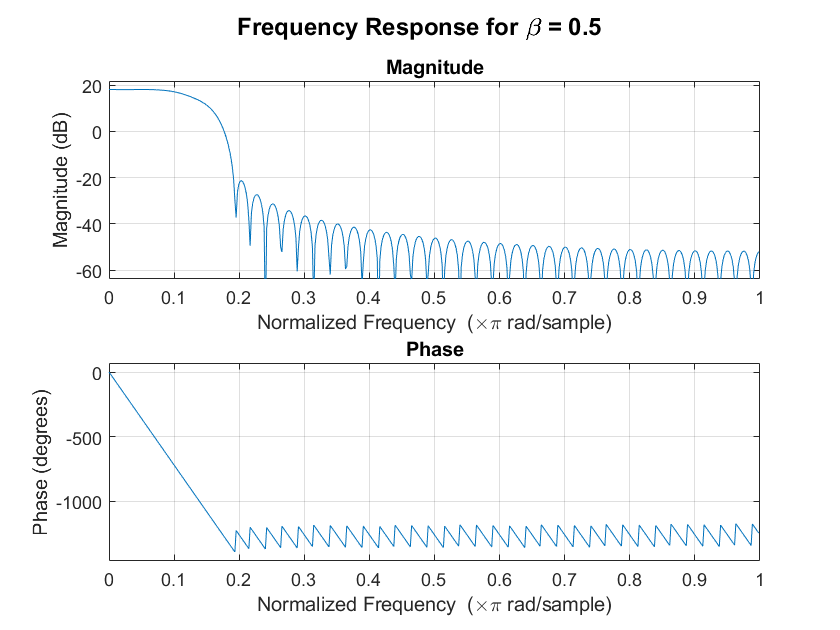
\includegraphics[width=0.5\textwidth]{srrc_freq_response_beta_0_5.png}}}
	\caption{SRRC Filter Frequency Response with $\beta=0.5$}
	\label{fig::srrc_freq_response_beta_0_5}
\end{figure}

\begin{figure}[H]
	\centerline{\fbox{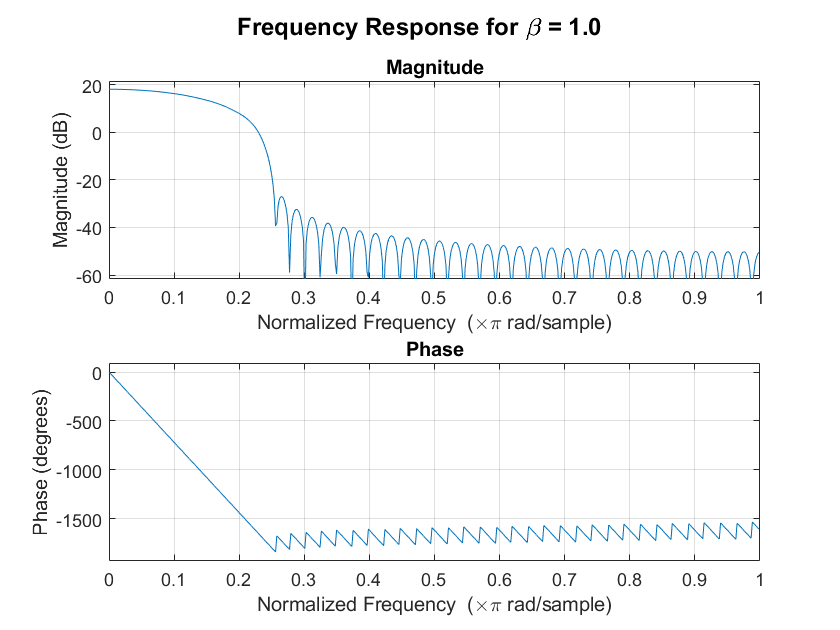
\includegraphics[width=0.5\textwidth]{srrc_freq_response_beta_1.png}}}
	\caption{SRRC Filter Frequency Response with $\beta=1$}
	\label{fig::srrc_freq_response_beta_1}
\end{figure}

\noindent Examining the frequency response of each of the filters, we see that the spectral efficiency is maximized for small values of the rolloff factor, $\beta$. However, the sharp filter transitions required for small $\beta$ increases the complexity of the filter. We can confirm this statement by plotting the impulse response of the filter with $\beta=0$ and $\beta=1$.

\begin{figure}[H]
	\centerline{\fbox{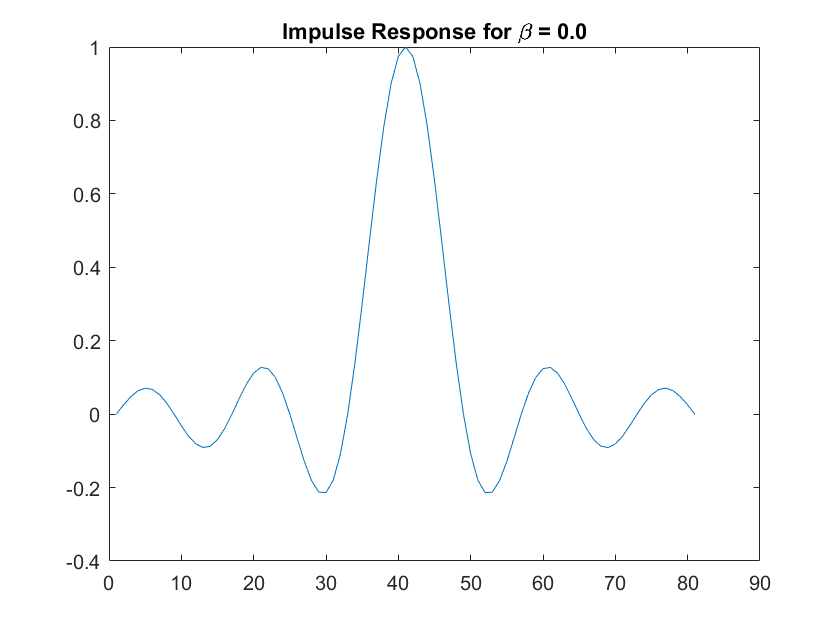
\includegraphics[width=0.5\textwidth]{srrc_impulse_response_beta_0.png}}}
	\caption{SRRC Filter Impulse Response with $\beta=0.0$}
	\label{fig::srrc_impulse_response_beta_0}
\end{figure}

\begin{figure}[H]
	\centerline{\fbox{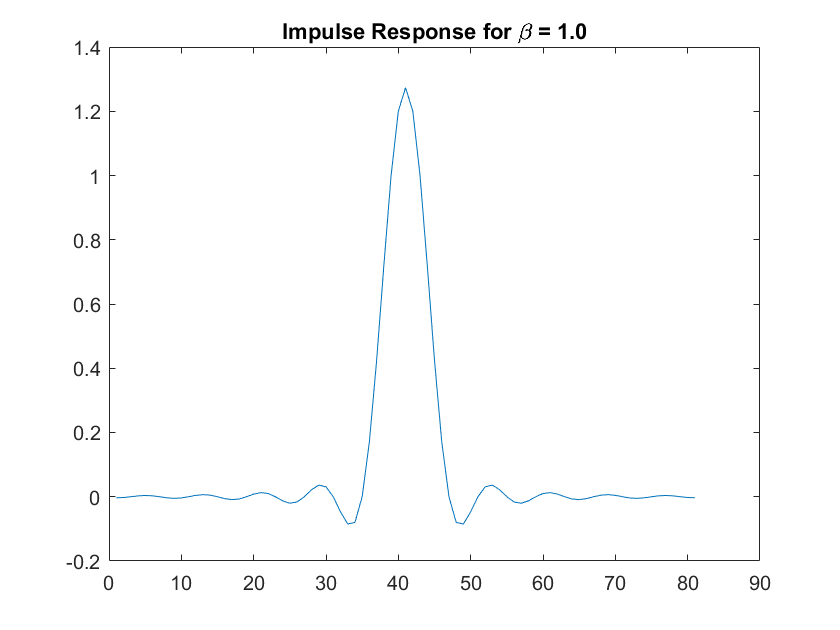
\includegraphics[width=0.5\textwidth]{srrc_impulse_response_beta_1.png}}}
	\caption{SRRC Filter Impulse Response with $\beta=1$}
	\label{fig::srrc_impulse_response_beta_1}
\end{figure}

\noindent Comparing the two impulses responses, we see that the impulse response with $\beta=1$ converges much faster than the impulse response with $\beta=0$. This allows us to truncate the impulse response sooner, which in turn reduces the filter length and complexity.


\section{Conclusion}
% Conclusions to the overall lab that discuss meaningful lessons learned and other takeaways from the assignment. (Important)
	
\end{document}